\documentclass[11pt,table]{article}

\usepackage{subfiles}
\usepackage[breakable]{tcolorbox}
%\usepackage{parskip} 

\usepackage{iftex}
\ifPDFTeX
\usepackage[T1]{fontenc}
\usepackage{mathpazo}
\else
\usepackage{fontspec}
\fi
\usepackage[english]{babel}
\usepackage{lipsum}
\usepackage{microtype}
\usepackage{float}
\usepackage{caption}


\usepackage{subcaption}
\usepackage[skip=50pt]{caption} % default 10pt
\captionsetup[figure]{skip=10pt}
\usepackage{rotating}
\usepackage{wrapfig}

\usepackage{graphicx}
\graphicspath{
  {figures/}
}  

\captionsetup{format=plain,
	aboveskip=-0.2cm,
	indention=0cm, 
	textformat=simple,
	textfont=small,
	labelfont=small, 
	justification=centering,
	labelfont=bf}



\usepackage[Export]{adjustbox} % Used to constrain images to a maximum size
\adjustboxset{max size={0.9\linewidth}{0.9\paperheight}}
\usepackage{float}
%\floatplacement{figure}{H} % forces figures to be placed at the correct location
\usepackage{xcolor}    % Allow colors to be defined
\usepackage{enumerate} % Needed for markdown enumerations to work
\usepackage{geometry}  % Used to adjust the document margins
\usepackage{amsmath}   % math symbols
\usepackage{amssymb}   % more math symbols
\usepackage{siunitx}   % write numbers and units nicely
% \usepackage{textcomp}  % defines textquotesingle
\usepackage[           % Literaturverwaltung mit BibLaTeX
  style=ieee,
  sorting=none
]{biblatex}                     
\addbibresource{bibliography.bib} % Pfad Literaturverzeichnis
\usepackage[autostyle=true]{csquotes} % Für BibLaTeX notwendig
\usepackage{upquote}   % Upright quotes for verbatim code
\usepackage{eurosym}   % defines \euro
% \usepackage[mathletters]{ucs} % Extended unicode (utf-8) support
\usepackage{fancyvrb}  % verbatim replacement that allows latex
\usepackage{grffile}   % extends the file name processing of package graphics 
% to support a larger range
\makeatletter % fix for grffile with XeLaTeX
\def\Gread@@xetex#1{%
	\IfFileExists{"\Gin@base".bb}%
	{\Gread@eps{\Gin@base.bb}}%
	{\Gread@@xetex@aux#1}%
}
\makeatother

\usepackage{hyperref}
\usepackage[capitalise]{cleveref}
\Crefname{figure}{Fig.}{Figs.}% {<type>}{<singular>}{<plural>}
\usepackage{acro}

% The default LaTeX title has an obnoxious amount of whitespace. By default,
% titling removes some of it. It also provides customization options.
\usepackage{titling}
\usepackage{longtable} 
\usepackage{booktabs}  
\renewcommand{\arraystretch}{1.2} % more space between table rows

\usepackage[inline]{enumitem}
\usepackage[normalem]{ulem}
% normalem makes italics be italics, not underlines
\usepackage{mathrsfs}

\captionsetup[table]{skip=10pt}


% Colors for the hyperref package
\definecolor{urlcolor}{rgb}{0,.145,.698}
\definecolor{linkcolor}{rgb}{0,0,0}%{.71,0.21,0.01}
\definecolor{citecolor}{rgb}{0,0,0}%{.12,.54,.11}


\title{Predicting Renewable Energy Production Using Machine Learning Methods}
\author{Luis Gentner, Leon Sengün, Dilara Yildiz}
\date{\today}



% Prevent overflowing lines due to hard-to-break entities
\sloppy 

\hypersetup{
	breaklinks=true,  % so long urls are correctly broken across lines
	colorlinks=true,
	urlcolor=urlcolor,
	linkcolor=linkcolor,
	citecolor=citecolor,
}
% Slightly bigger margins than the latex defaults

\geometry{verbose,tmargin=1in,bmargin=1in,lmargin=1in,rmargin=1in}

\newcommand{\ket}[1]{\left|{#1}\right\rangle}
\newcommand{\bra}[1]{\left\langle{#1}\right|}
\newcommand{\braket}[2]{\left\langle{#1}\middle|{#2}\right\rangle}



\usepackage{fancyhdr}
\addtolength{\headheight}{1.2cm} % make more space for the header
\pagestyle{fancy} %plain} % use fancy for all pages except chapter start
\fancyhead[L]{\leftmark}
%\lhead{\includegraphics[height=1.3cm]{logo2}} % left logo
\rhead{
\includegraphics[height=0.6cm]{header.png}}   % right logo
%\renewcommand{\headrulewidth}{0pt} % remove rule below header


\title{Project Title}
\author{Luis Gentner, Leon Sengün, Dilara Yildiz}
\date{\today}



\begin{document}
\begin{titlepage} 
	\centering 
	\rule{\textwidth}{1pt} 
	\vspace{2pt}\vspace{-\baselineskip} 
	\rule{\textwidth}{0.4pt} 
	\vspace{0.1\textheight} 
	
	
	%%% Adjust your project title here
	{\Huge PREDICTING RENEWABLE ENERGY }\\[0.5\baselineskip] 
	{\Huge PRODUCTION USING }\\[0.5\baselineskip]
	%{\Large }\\[0.5\baselineskip] 
	{\Huge MACHINE LEARNING METHODS} 
	
	
	\vspace{0.025\textheight} 
	\rule{0.3\textwidth}{0.4pt} 
	\vspace{0.1\textheight}
	
	%%% Your names, if long, a "\\" in between may help to make things look better
	{\Large \textsc{Luis Gentner, Leon Sengün, Dilara Yildiz}} 
	
	\vfill 
	
	%%% You can include a nice image from your project here
	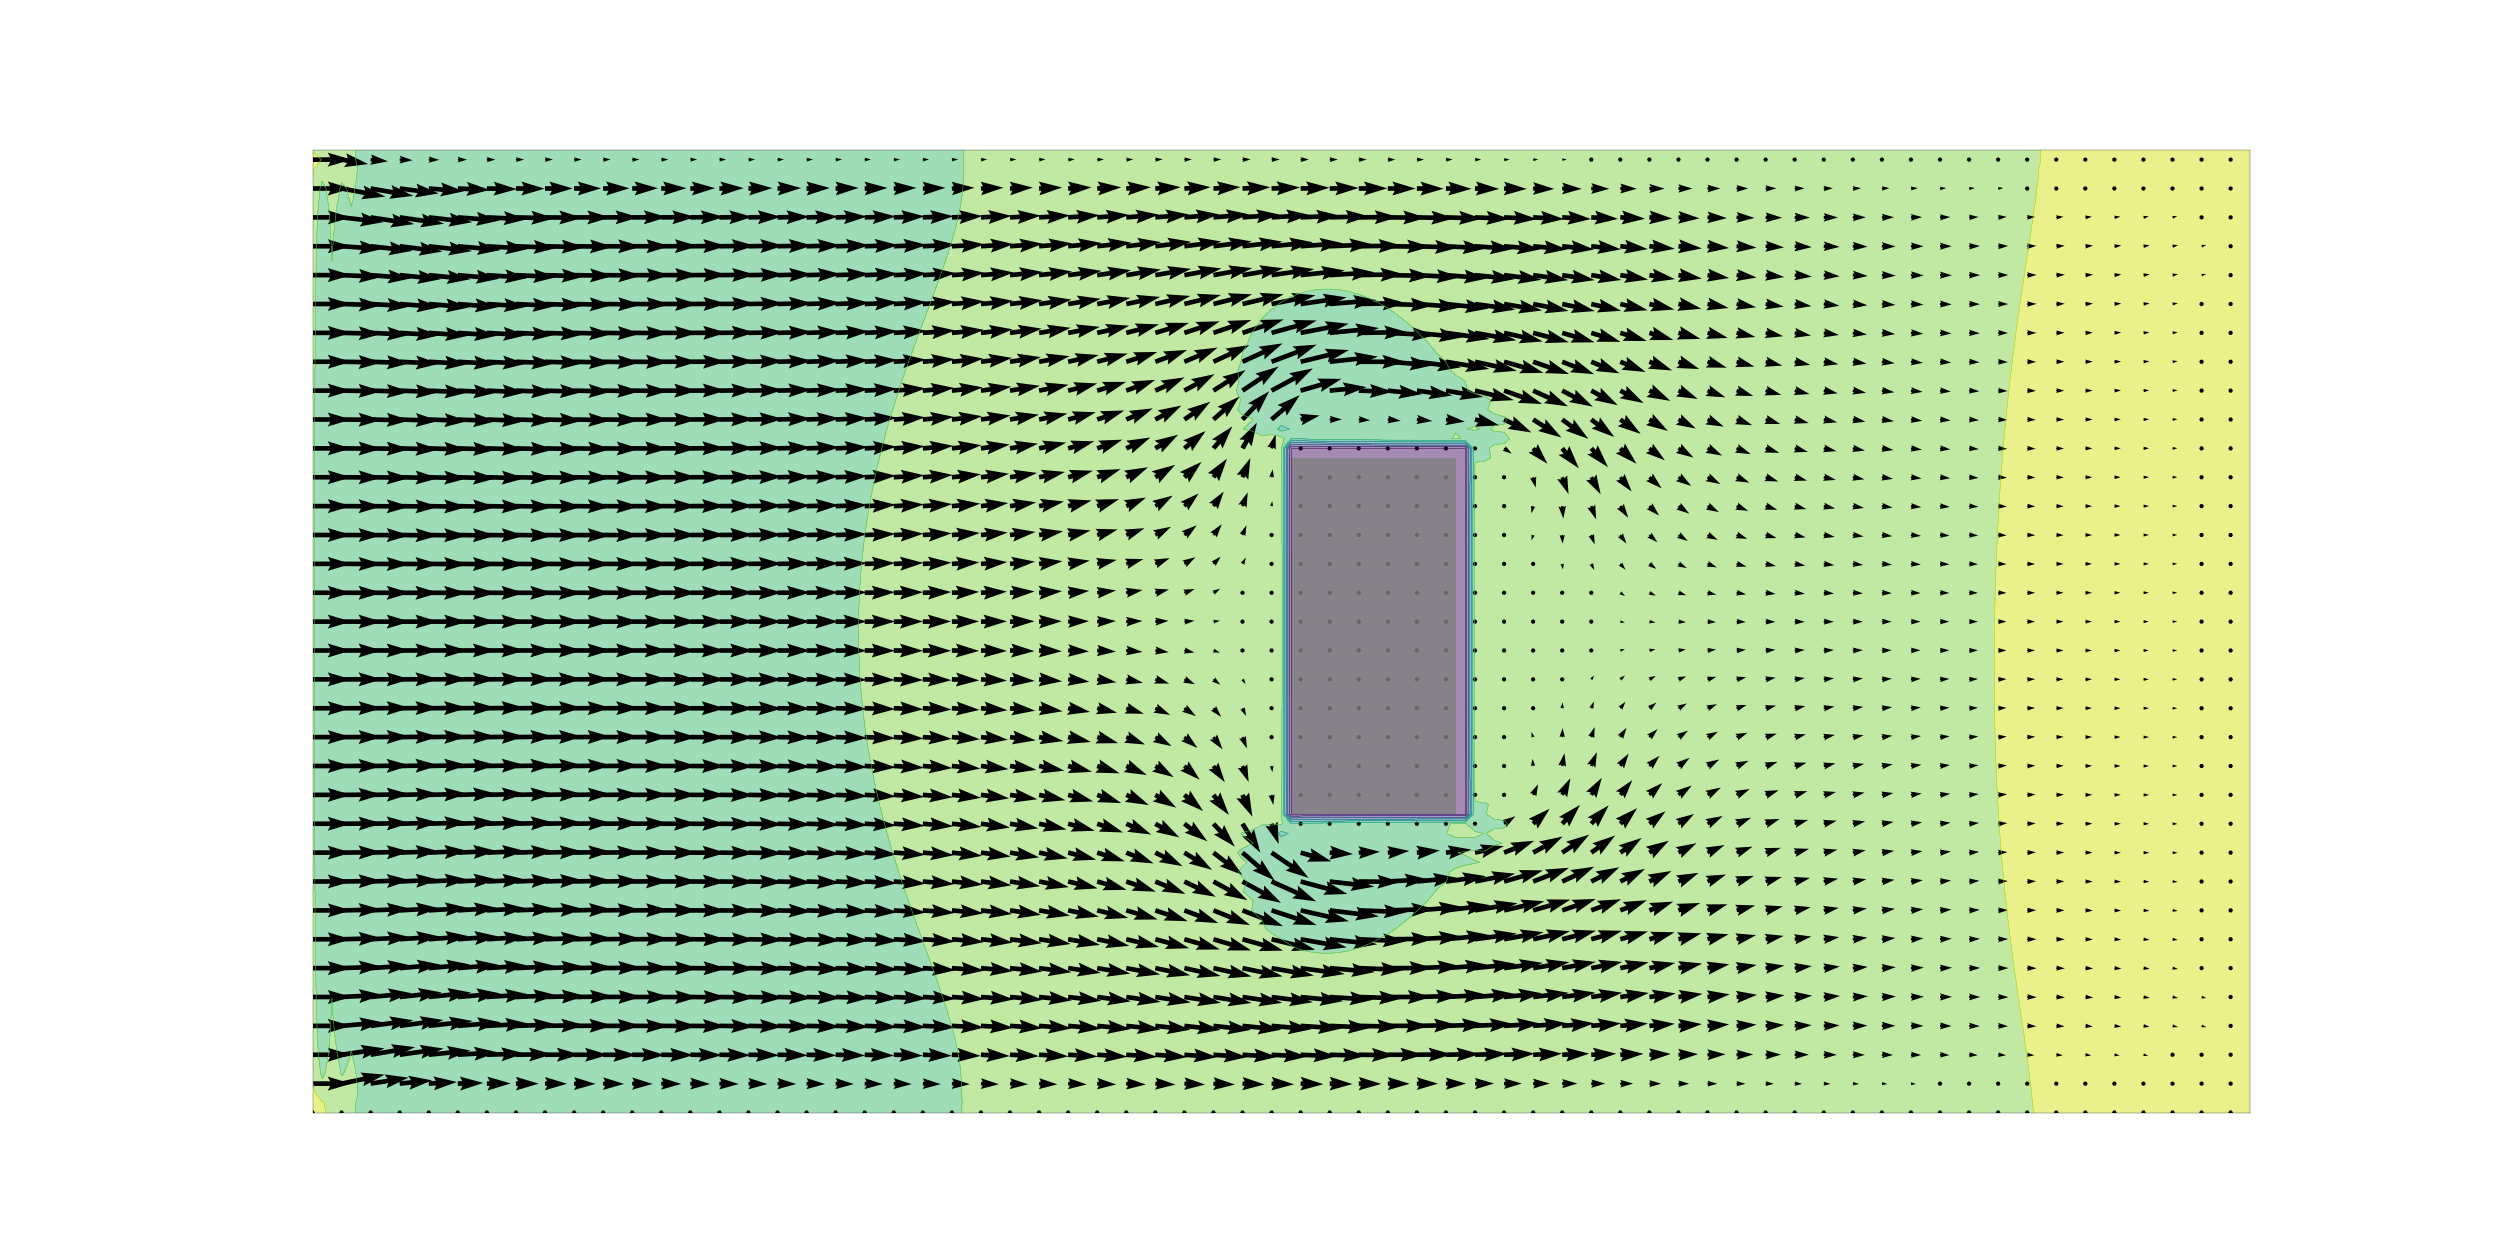
\includegraphics[width=0.5\linewidth]{Figures/example_cover.png} \\
	\vspace{0.05\textheight}
	{\large\textsc{Machine Learning Methods in Mechanics \\Report}\\ -\\ University of Stuttgart} 
	
	
	\vspace{0.1\textheight} 
	
	%%% Adjust the date here if you like
	{\normalsize \today}
	
	
	\rule{\textwidth}{0.4pt}
	\vspace{2pt}\vspace{-\baselineskip}
	\rule{\textwidth}{1pt}
	
\end{titlepage}

\pagenumbering{roman}

\newpage

\tableofcontents

\newpage

\pagenumbering{arabic}

%%% The following structure is a suggestion
%%% If you prefer to use your own, you can change everything
\section{Introduction}

The increase in the share of renewable energy sources in total energy production leads to a increasingly fluctuating power generation. Therefore, measures for a stable energy supply will gain importance. Information about future energy production could enable power plant operators to control their power production up and down in order to match the incoming renewable energy. A future prediction could also help to store energy in a targeted manner. 
With this background, the goal of this work is to develop a machine learning model that predicts the renewable energy production 12 hours into the future.\\
There is a variety of model architectures for this problem, including CNNs (Convolutional Neural Networks), RNNs (Recurrent Neural Networks), Autoencoders, GRUs (Gated Recurrent Units) or LSTMs (Long Short Term Memory). This paper will first explore and evaluate existing models regarding their accuracy, then iteratively develop an advanced and optimized model architecture.\\

Description of the project. Images are always a plus. You should reference each figure in the text and explain what can be seen. The flow field shows particle velocities. It is taken from~\cite{Author2020}. What is the problem? What is the goal? What is your idea?\\ 

%\lipsum[2]

You can include wrapped figures and tables, like Table~\ref{tab:features}. To make it work, there should be no newlines between the wrapped table or figure and the surrounding text. Normal tables work just as usual, like in Table~\ref{tab:other_parameters}.\\
%\lipsum[1]

%\begin{wraptable}{r}{0.55\textwidth}
%	%\begin{table}[]
%	%\centering
%	%\vspace{0pt}
%	\begin{tabular}{@{} lrrrrrr @{}}
%		\toprule
%		 & $L$ & $\lambda^S$ & $\mu^S$ & $k_{0\text{S}}^{\text{F}1}$ & $k_{0\text{S}}^{\text{F}2}$ & $k_{0\text{S}}^{\text{F}3}$ \\
%		\midrule
%		min & 0.6 & 3.1 & 15.8 & 0.1 & 0.003 & 0.1 \\
%		max & 8.3 & 196.8 & 285.5 & 1.0 & 0.1 & 0.9 \\
%		example & 1.33 & 21 & 126 & 0.18 & 0.05 & 0.23 \\
%		\bottomrule
%	\end{tabular}
%	\caption{Feature values used for training the CNN.}\label{tab:features}
%\end{wraptable} 

%\lipsum[2-3]


%\begin{table}[]
%	\centering
%	%\vspace{0pt}
%	\begin{tabular}{@{} lrrrrrr @{}} 
%		\toprule
%		 & $L$ & $\lambda^S$ & $\mu^S$ & $k_{0\text{S}}^{\text{F}1}$ & $k_{0\text{S}}^{\text{F}2}$ & $k_{0\text{S}}^{\text{F}3}$ \\
%		\midrule
%		min & 0.6 & 3.1 & 15.8 & 0.1 & 0.003 & 0.1 \\
%		max & 8.3 & 196.8 & 285.5 & 1.0 & 0.1 & 0.9 \\
%		example & 1.33 & 21 & 126 & 0.18 & 0.05 & 0.23 \\
%		\bottomrule
%	\end{tabular}
%	\caption{Values used to create the simulation in Figure~\ref{fig:flow}.}\label{tab:other_parameters}
%\end{table}

\section{Data and Feature Engineering}
In order to predict future energy production from renewable sources, data showing energy production in recent years is needed. Old data sets are not representative because the number of solar and wind power plants in operation has increased significantly in recent years.(\textbf{Zitat}) Therefore, years 2017-2021 were selected for neural network training in this paper. \\
Future solar and wind energy generation depends not only on past energy generation, but also on weather conditions. To account for this, a second dataset of past-year weather information (2017-2021) was chosen as an optional additional input to the models.
The following data sets were used in this paper:

\begin{itemize}
  \item Electricity data (2017-2021) obtained from Energy-Charts (from Fraunhofer ISE), hourly resolution
  \item Weather data (2017-2021) from DWD (Deutscher Wetterdienst) including 468 meteorological station in Germany, hourly resolution
\end{itemize}%

\subsection{Feature Engineering}
Raw data cannot necessarily be included directly as a feature in the model. Different pre-processing steps and a thoughtful selection of features can significantly improve the final result. 

\begin{figure}[h!]
	\centering
	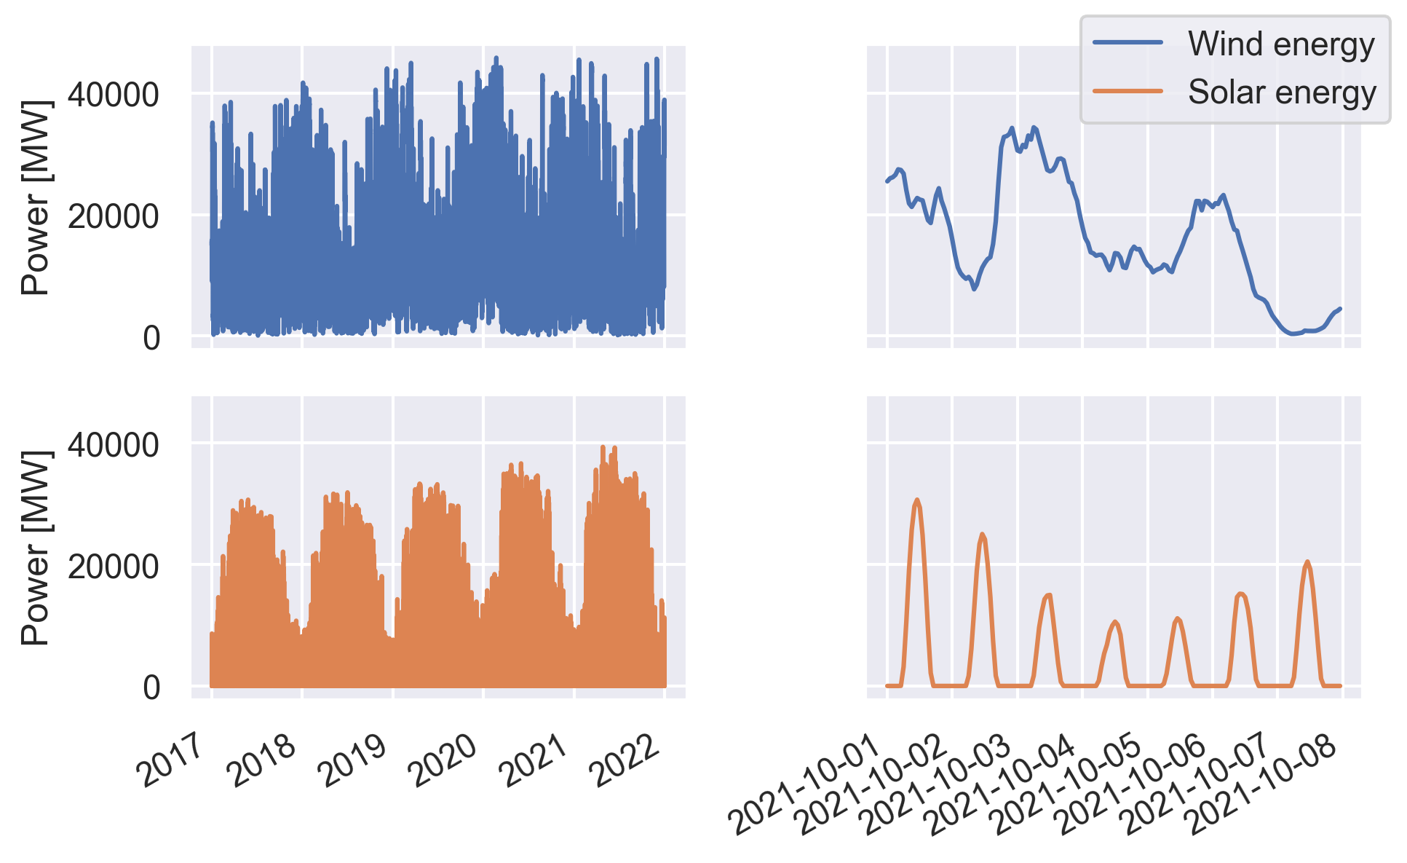
\includegraphics[scale=0.9]{Figures/electrData.png}
	\caption{Wind and solar energy production 2017-2021}
	\label{fig:electrData}
\end{figure}

Figure~\ref{fig:electrData} shows the wind and solar energy production of 2017-2021. Seasonal and daily fluctuations can be observed. To further investigate this phenomenon, a fourier analysis, shown in figure \ref{fig:fourier} was performed.

\begin{figure}[H]
\centering
\begin{subfigure}{.5\textwidth}
  \centering
  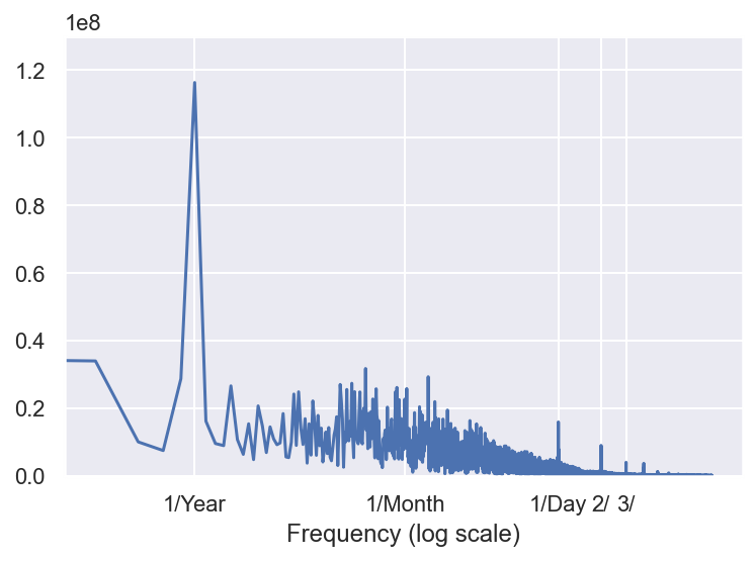
\includegraphics[width=0.9\linewidth]{Figures/fourierWind.png}
  \label{fig:fourierWind}
  \caption{Fourier analysis of wind energy production}
\end{subfigure}%
\begin{subfigure}{.5\textwidth}
  \centering
  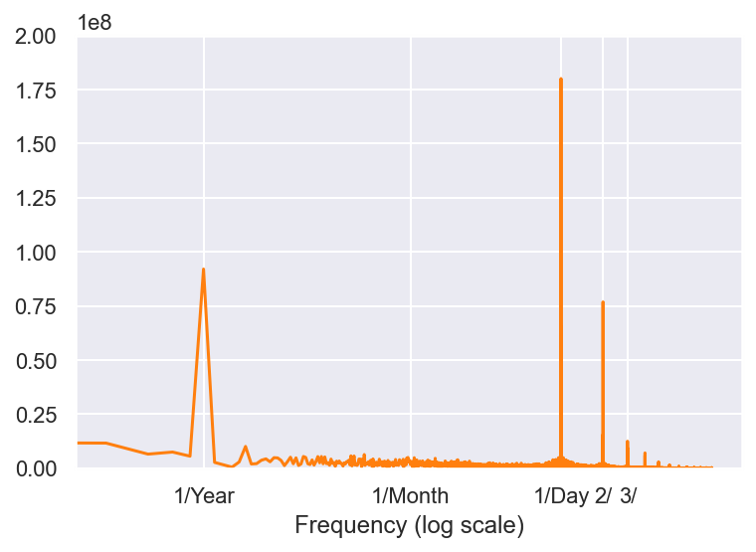
\includegraphics[width=0.9\linewidth]{Figures/fourierSolar.png}
  \label{fig:fourierSolar}
  \caption{Fourier analysis of solar energy production}
\end{subfigure}
\caption{Fourier analysis of electricity data}
\label{fig:fourier}
\end{figure}

The fourier analysis reveals the frequencys that appear in the wind/solar energy production data. The solar energy production shows the highest peak at a frequency of 1/day, matching the daily elevation of the sun. For both, wind and solar energy the yearly and daily fluctuations are dominant.\\
To account for these two frequencies, time is mapped to sine and cosine functions representing the periodicity of year and day (Figure~\ref{fig:timeSignal}). In addition, the solar elevation is determined, which, as expected, correlates strongly with solar energy production. The bottom plot in Figure~\ref{fig:timeSignal} shows the actual solar elevation by truncating the previous solar elevation curve to zero. In this way, the lack of sunlight during night is represented.

\begin{figure}[H]
	\centering
	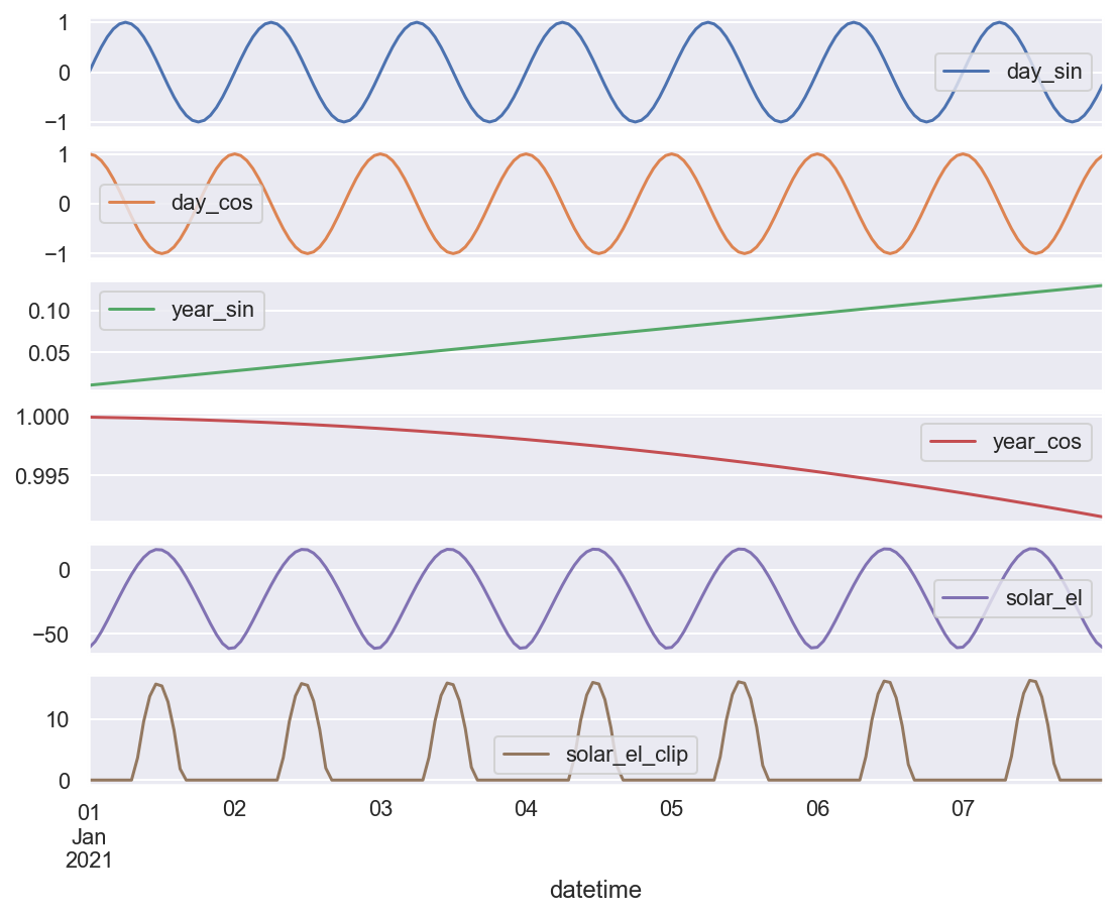
\includegraphics[scale=0.7]{Figures/timeSignal.png}
	\caption{Periodic features}
	\label{fig:timeSignal}
\end{figure}

The modified time features as well as air pressure, sunshine duration, temperature and wind speed were subjected to a correlation analysis. 

\begin{figure}[H]
	\centering
	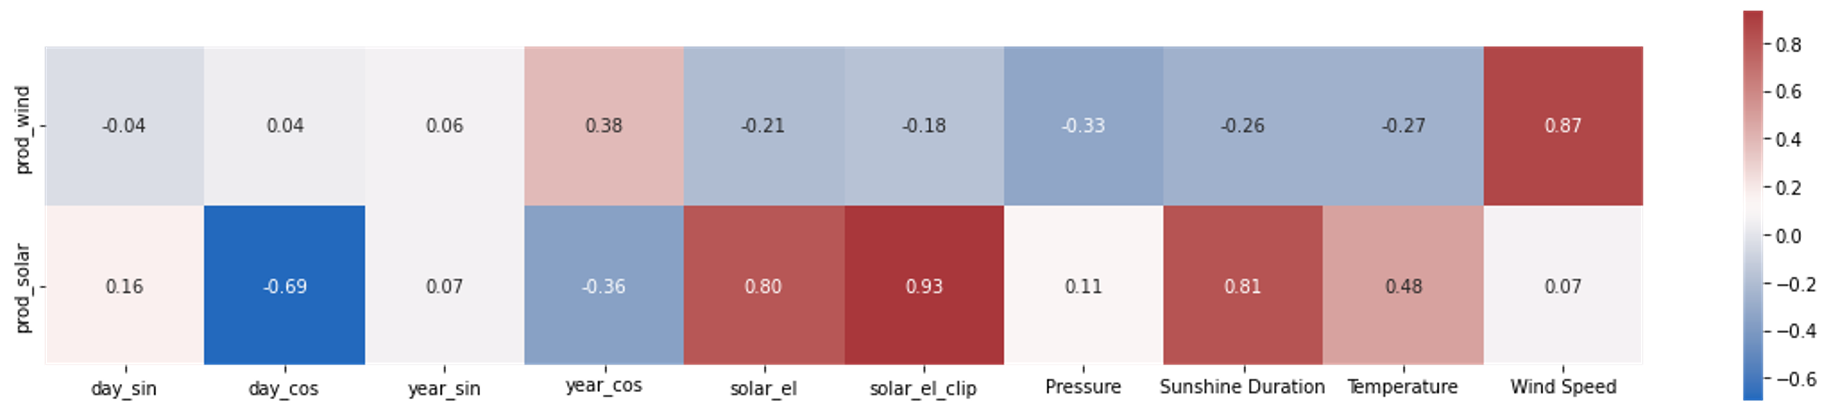
\includegraphics[scale=1]{Figures/correlation.png}
	\caption{Correlation analysis}
	\label{fig:correlation}
\end{figure}

Figure~\ref{fig:correlation} shows the correlation matrix. Darker colors indicate a higher (anti-)correlation. The solar energy production is strongly correlated to the cosine of the day, sunshine duration, temperature and clipped solar elevation. In contrast, wind energy production is only strongly correlated with wind speed and slightly correlated with pressure and temperature, which can be explained by the ideal gas equation. Although the sine of day and year do not hold a high correlation, they were included in the feature vector for completeness.

The final feature vector is a combination of two energy production features, six analytically determined time and solar elevation features, and 4 weather features (per weather station) as displayed in Table~\ref{tab:feature}.

\begin{table}[]
\begin{center}
\begin{tabular}{p{4.5cm}|p{5cm}|p{4.5cm}}
\toprule
\textbf{Energy Production} & \textbf{Time and Solar Elevation} & \textbf{Weather}              \\
\midrule
solar energy prod. & day sine                 & temperature          \\
wind energy prod.  & day cosine               & windspeed            \\
                   & year sine                & pressure             \\
                   & year cosine              & sunshine duration    \\
                   & solar elevation          &                      \\
                   & clipped solar elevation  &                     \\ \bottomrule
\end{tabular}
\end{center}
\caption{Features}
\label{tab:features}
\end{table}

Of 468 meteorological stations in Germany, only 117 provide reliable data (2017-2021). Of these remaining stations, 12 were selected for further representation of German weather. Decisive for the selection was the spatial proximity to offshore and solar installations as well as a broad distribution across Germany. The final weather stations are displayed on~\ref{fig:weatherStations}
\begin{figure}[H]
	\centering
	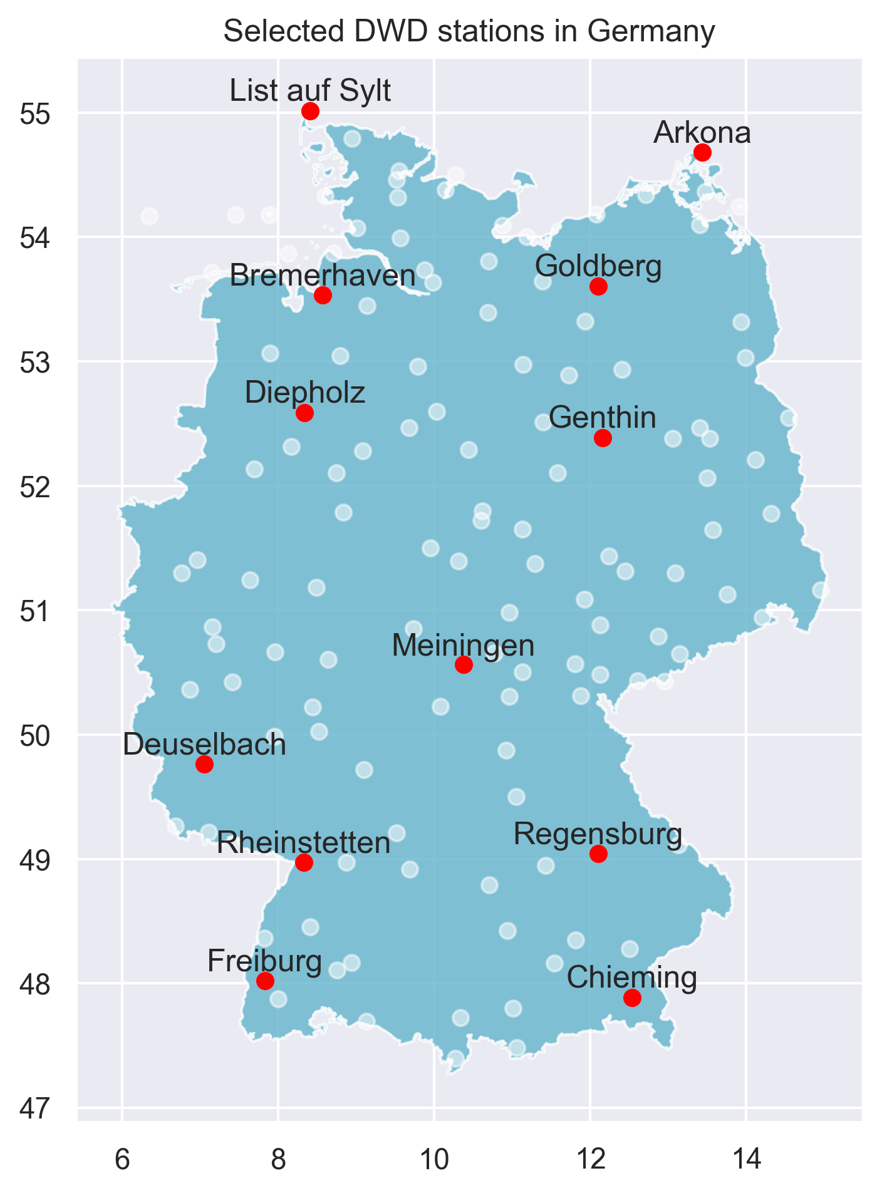
\includegraphics[scale=0.5]{Figures/weatherStations.png}
	\caption{Selected weather stations in Germany}
	\label{fig:weatherStations}
\end{figure}

\section{Methods and Model Architectures}

The goal of this work is to predict solar and wind energy production 12 hours into the future. Current research offers a variety of machine learning models for this problem. Therefore, as a first step, different models were applied to the problem and evaluated regarding their prediction accuracy. Unpromising approaches were then discarded while succesful models were further explored and improved.

The following models were investigated:

\begin{itemize}
\item \textbf{Repeat last Step:} This model only repeats the last given timestep, leading to a constant solar and wind energy production level in the future. As expected the model shows poor results. 
\item \textbf{Repeat Yesterday:} Here the course of yesterday, starting at the same time, is repeated. 
\item \textbf{Linear:} This architecture depicts a linear relation inducing a higher accuracy.
\item \textbf{Dense Layer:} While the first three models did not use any machine learning techniques, this architecture uses 512 neurons in a dense layer. The result is an increase in the R$^2$ score up to 0.84.
\item \textbf{CNN:} Convolutional Neural Network with 3x256 and 25x256
\item \textbf{SRNN:} Simple Recurrent Neural Network with 32 units
\item \textbf{GRU:} Gatet Recurrent Units with 32 units
\item \textbf{LSTM 32:} Long Short Term Memory network with 32 units
\item \textbf{LSTM 32$^2$:} Long Short Term Memory network with two layers each containing 32 units
\end{itemize}


\begin{figure}[H]
	\centering
	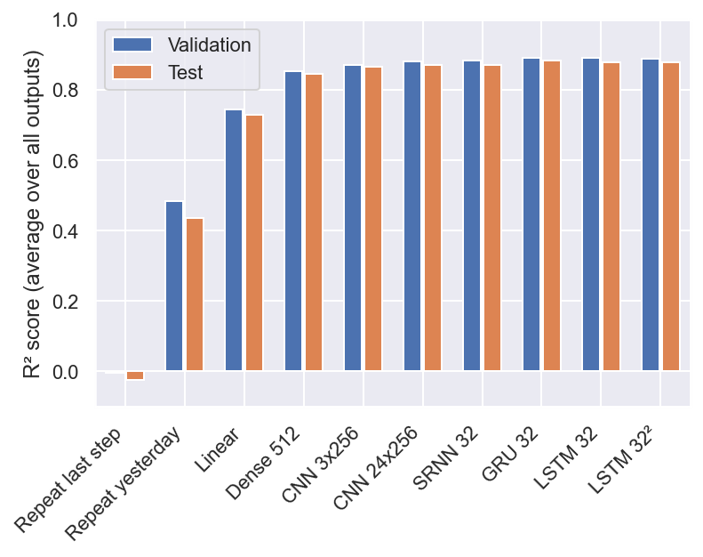
\includegraphics[scale=0.6]{Figures/benchmarks.png}
	\caption{Iterative model development}
	\label{fig:benchmarks}
\end{figure} 

\begin{figure}[H]
	\centering
	
\includegraphics[scale=1]{Figures/modelEvolution.png}
	\caption{Iterative model development}
	\label{fig:modelEvo}
\end{figure}

\begin{figure}[H]
	\centering
	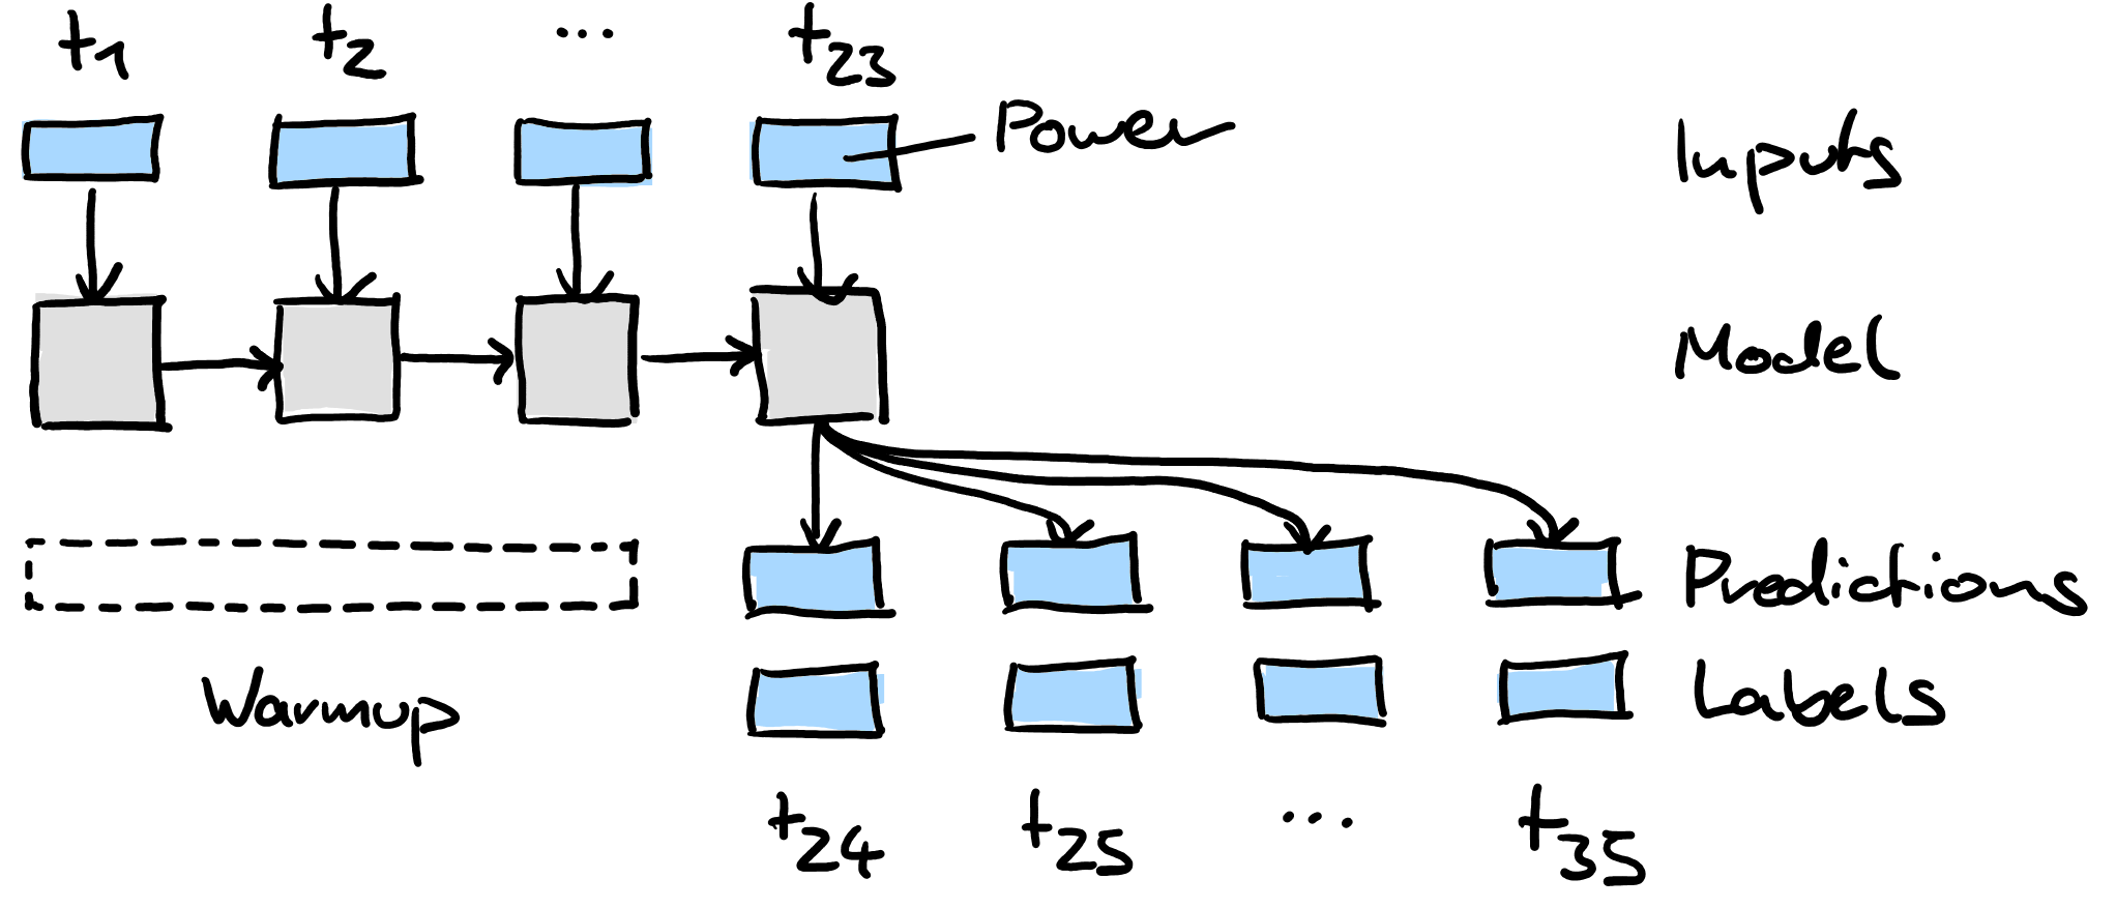
\includegraphics[scale=1]{Figures/SRNN.png}
	\caption{Simple recurrent neural network (SRNN)}
	\label{fig:SRNN}
\end{figure}

\begin{figure}[H]
	\centering
	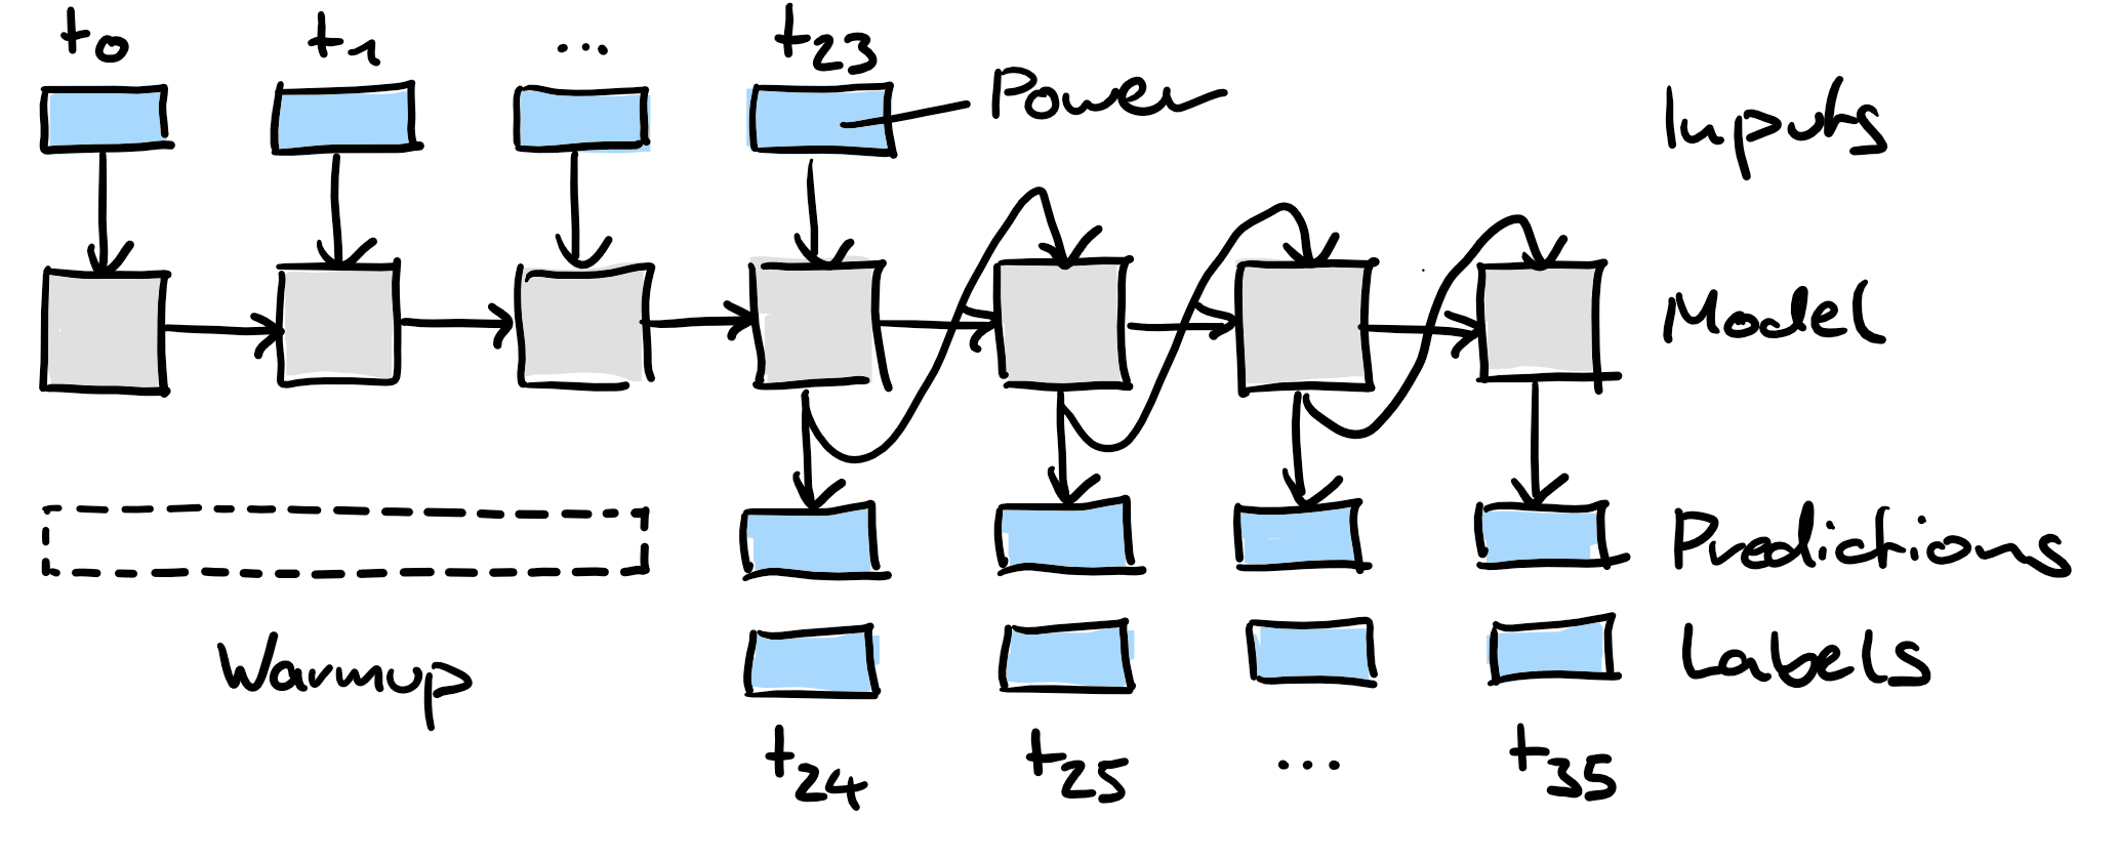
\includegraphics[scale=1]{Figures/ARNN.png}
	\caption{Autoregressive recurrent neural network (ARNN)}
	\label{fig:ARNN}
\end{figure}

\begin{figure}[H]
	\centering
	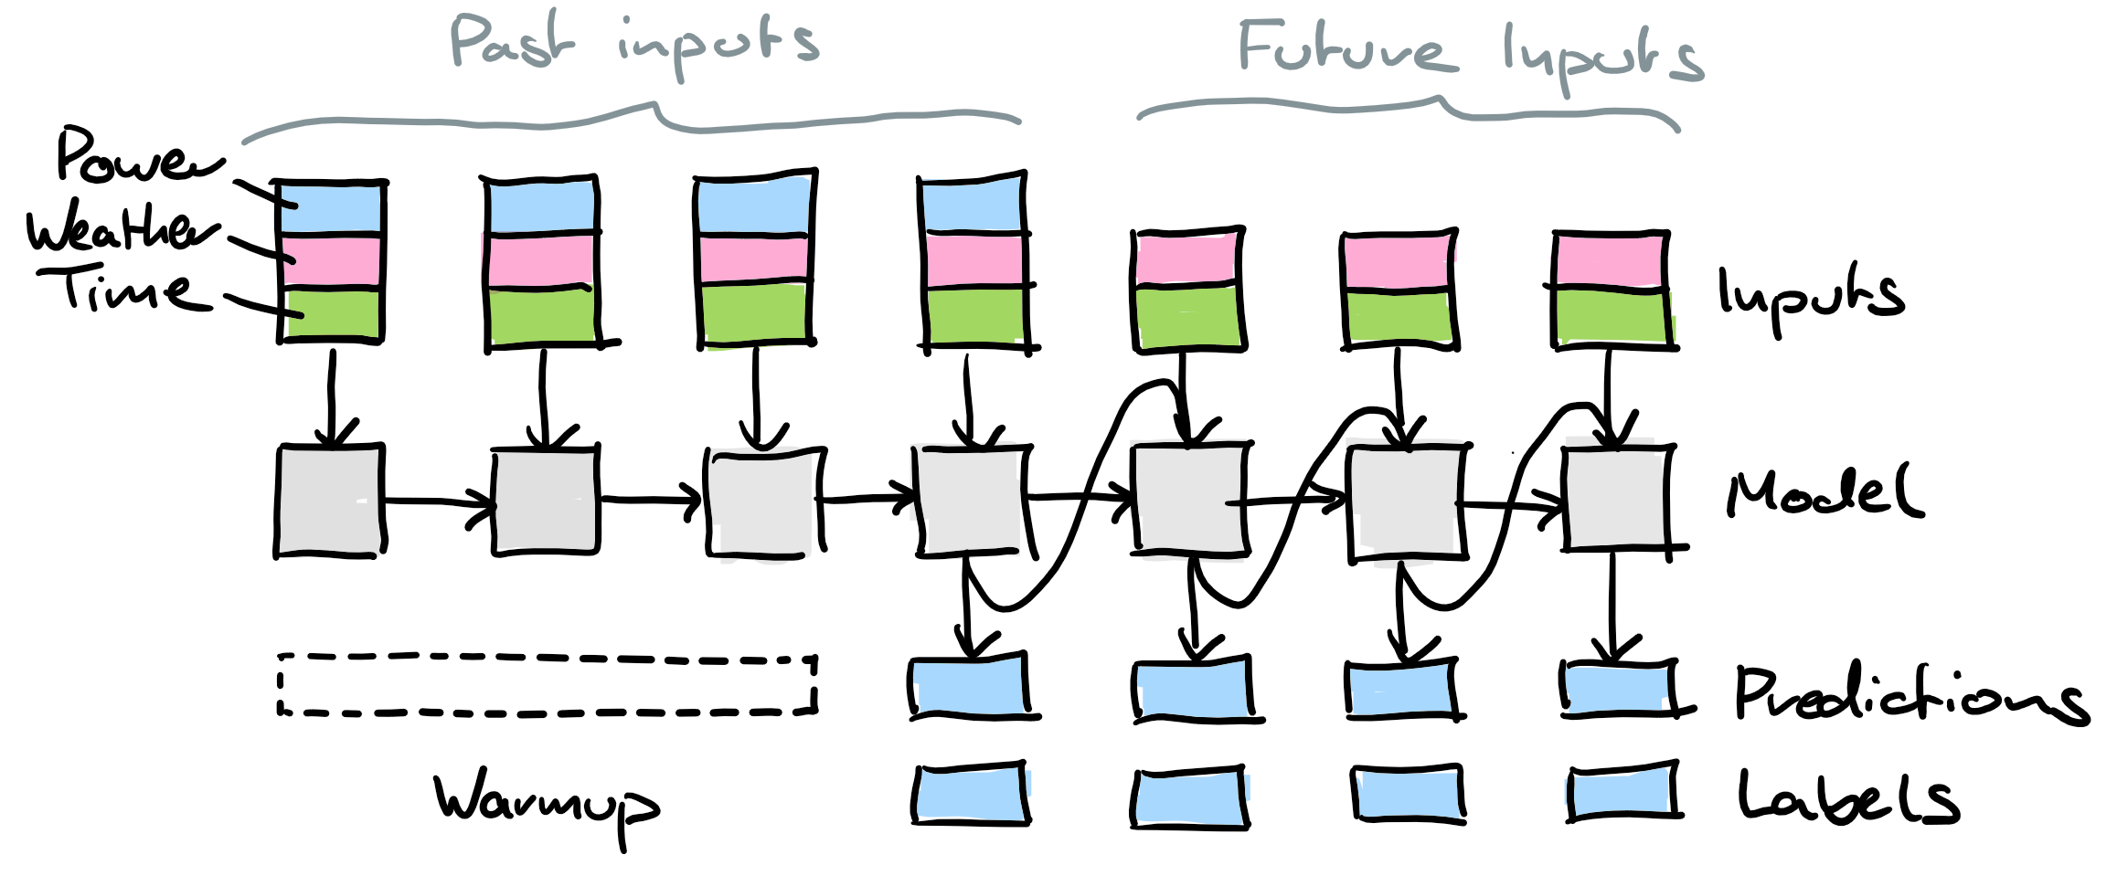
\includegraphics[scale=1]{Figures/continousARNN.png}
	\caption{Continous autoregressive recurrent neural network}
	\label{fig:continousARNN}
\end{figure}

\section{Results and Optimization}
\section{Conclusion}
\section{Outlook}

\subsection{The Navier-Stokes-Equations}

Equations as usual, like in Equation~\ref{equ:max_entropy}. Recall that equations like

\begin{equation}\label{equ:max_entropy}
	\phi_\mathrm{max} = \max_{\theta} \left[ \log(\sin(\theta - \exp(\theta))) - \theta^2 \right]
\end{equation}

are part of the text and should be treated like a word.

%\lipsum[1]

Or without numbering, like the realtivistic kinetic energy 

\begin{equation*}
	E = \frac{mc^2}{\sqrt{1 - \frac{v^2}{c^2}}},
\end{equation*}

which yields the Newtonian kinetic energy $E = \frac 1 2 m v^2$ when linearized for small velocities $v$.

\subsection{Solution Method}
%\lipsum[3-4]
\begin{wrapfigure}{r}{0.55\textwidth}
	\centering
	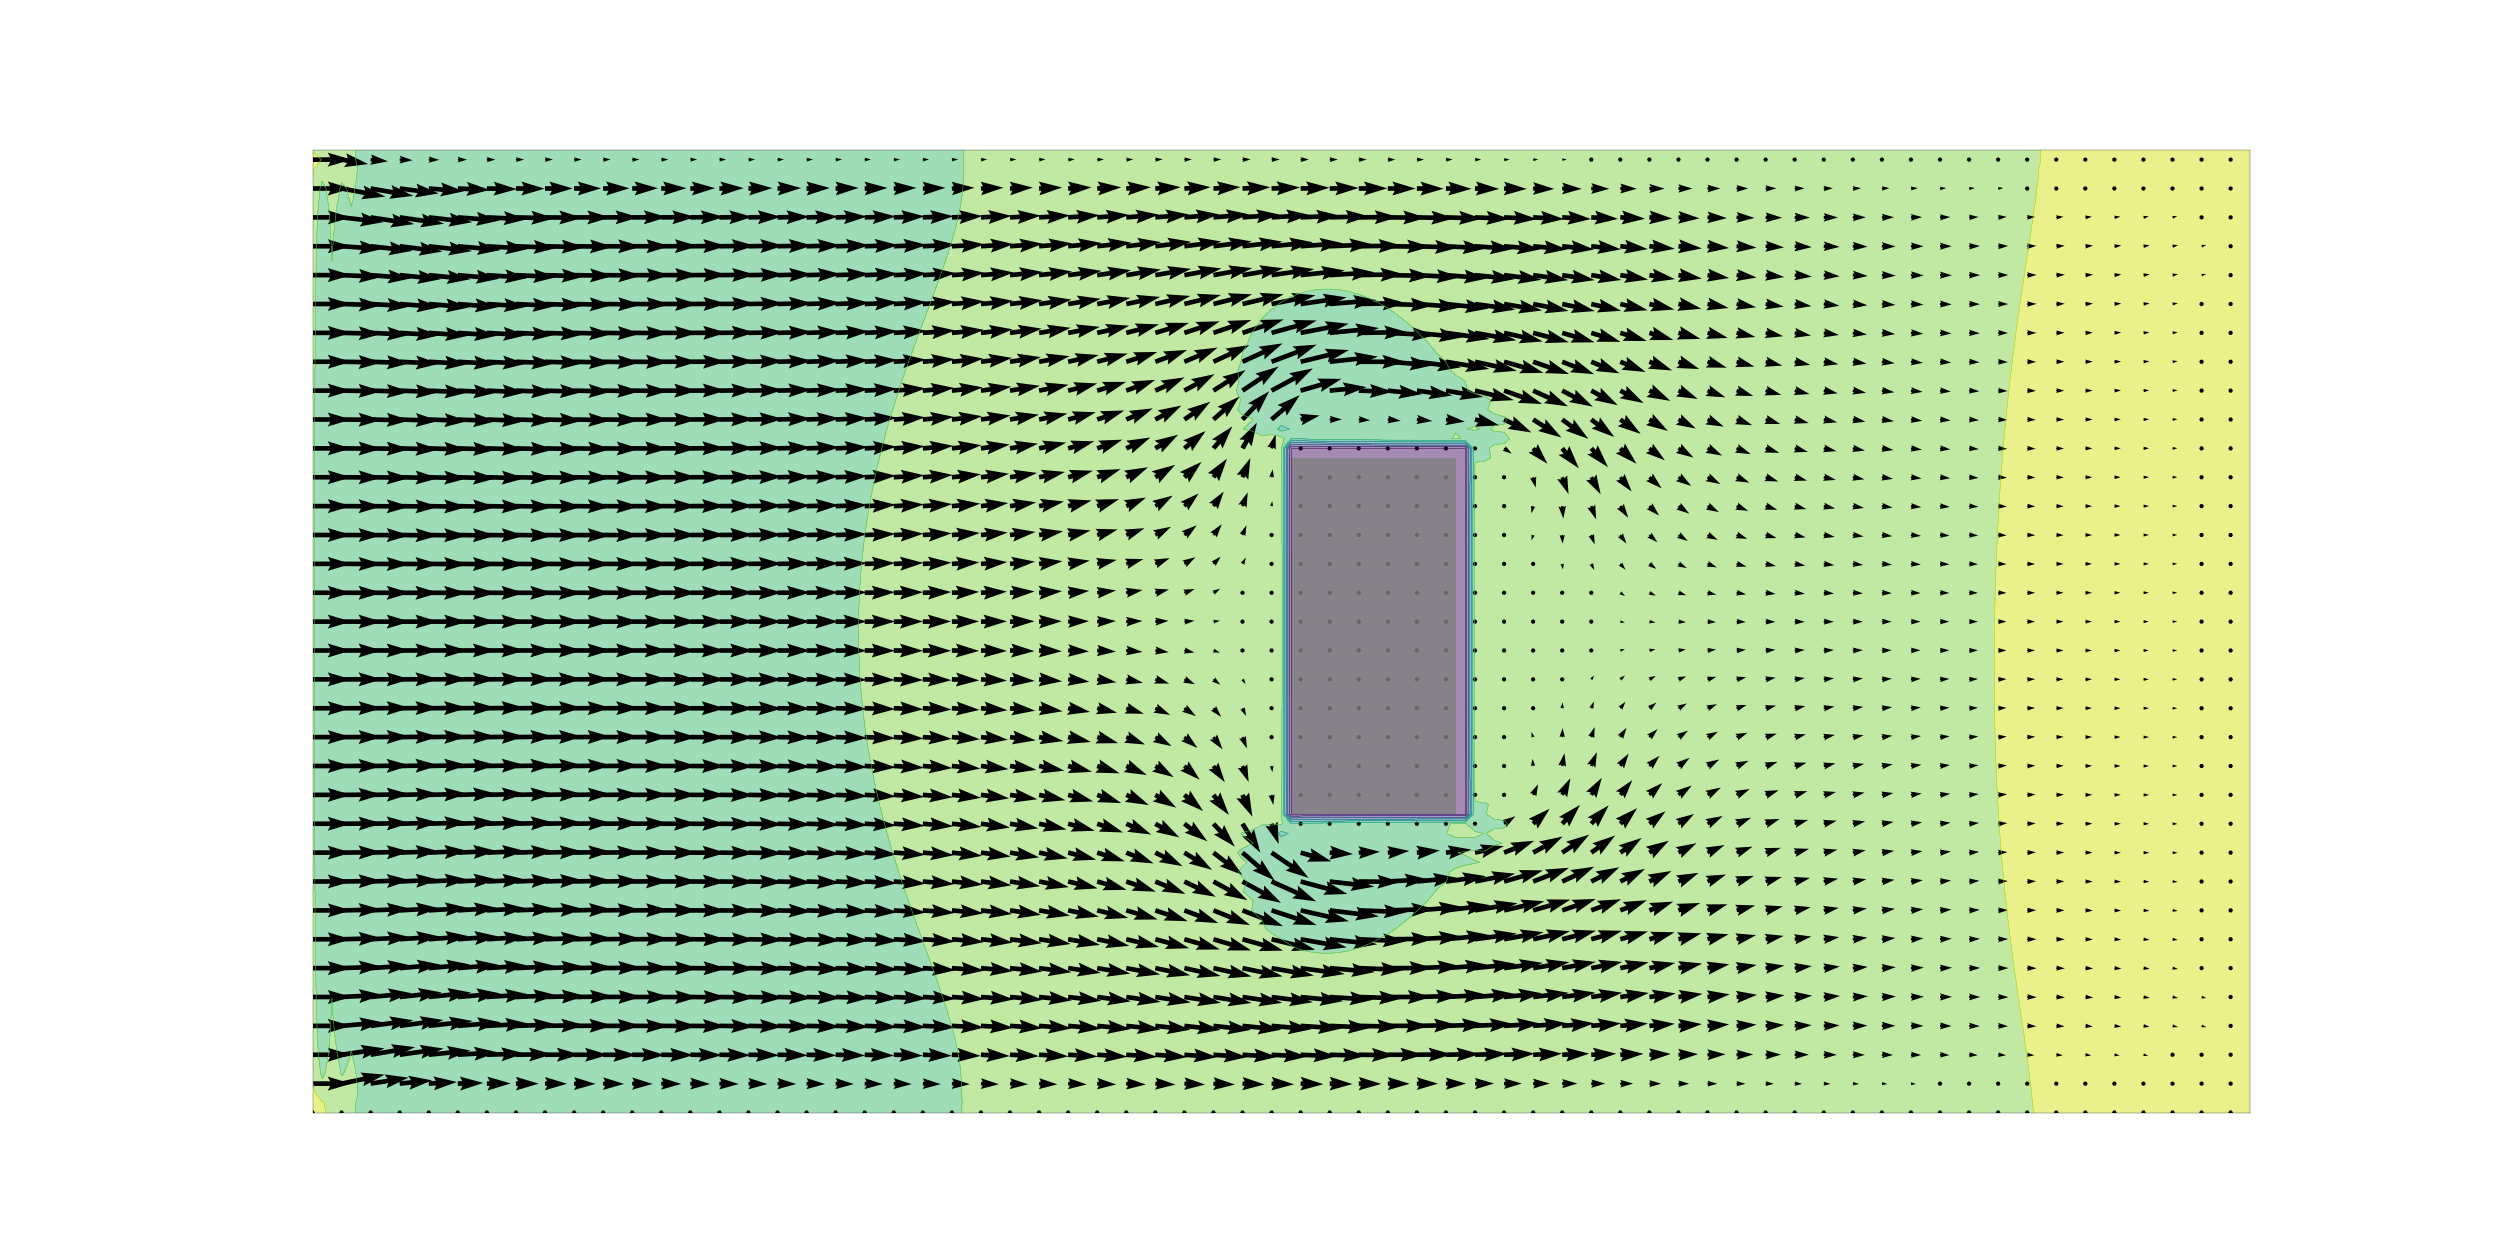
\includegraphics[scale=1.0]{Figures/example_cover.png}
	\caption{You can also use wrapped figures like this.}
	\label{fig:wrapfigure_example}
\end{wrapfigure}
%\lipsum[5] \\ \newline
Figure~\ref{fig:wrapfigure_example} shows how to include wrapped figures that text can float around. Depending on what is depicted and how large it is, it may look better than a full figure.

\section{Convolutional Neural Networks}

%\lipsum

\section{Idea and Data Generation}

%\lipsum

\section{Results}

%\lipsum

\begin{footnotesize}
\bibliographystyle{acm}


%%% This builds the bibliography
%%% You can use either bibtex with the following line and the "bibliography.bib" file
%%% OR ALTERNATIVELY comment the next line and uncomment the "thebibliography" environment

\bibliography{bibliography}

%%% comment the line above and uncomment the lines below
%%% for manually creating the bibliography

%\begin{thebibliography}{1}
%	
%	\bibitem{Author2020}% 
%	\textsc{A.\,W.~Harrow, A.~Hassidim, and S.~Lloyd},
%	\emph{Physical review letters 113} (15), 150502, (2009)
%	
%	\bibitem{Author2012}% 
%	\textsc{A.\,Y.~Kitaev},
%	\emph{Russian Mathematical Surveys 52} (6) p.\,1191--1249, (1997)
%	
%	
%\end{thebibliography}


\end{footnotesize}


%\newpage

\end{document}
